% Gemini theme
% https://github.com/anishathalye/gemini

\documentclass[final]{beamer}

% ====================
% Packages
% ====================

\usepackage[T1]{fontenc}
\usepackage{lmodern}
\usepackage[size=custom,width=118,height=84,scale=1.4]{beamerposter}
\usetheme{gemini}
%% \usefonttheme{professionalfonts}
%% \usefonttheme{serif}
%% \usecolortheme{gemini}
\usepackage{graphicx}
\usepackage{booktabs}
\usepackage{eso-pic}
\usepackage{amsmath,amssymb,bm}

% ====================
% Lengths
% ====================

% If you have N columns, choose \sepwidth and \colwidth such that
% (N+1)*\sepwidth + N*\colwidth = \paperwidth
\newlength{\sepwidth}
\newlength{\colwidth}
\setlength{\sepwidth}{0.025\paperwidth}
\setlength{\colwidth}{0.3\paperwidth}

\newcommand{\separatorcolumn}{\begin{column}{\sepwidth}\end{column}}

% ====================
% Title
% ====================

\title{Low SNR Multiframe Registration for Cubesats}
\AddToShipoutPictureFG*{
\AtPageUpperLeft{\put(-60,-80){\makebox[\paperwidth][r]{Paper \#3337}}}
}%

\author{Evan Widloski \and Farzad Kamalabadi}

\institute[shortinst]{University of Illinois Urbana-Champaign}

% ====================
% Footer (optional)
% ====================

\footercontent{
  CSLSC, Champaign IL \,
  \href{mailto:evan\_icip@widloski.com}{evan\_icip@widloski.com}}
% (can be left out to remove footer)

% ====================
% Logo (optional)
% ====================

% use this to include logos on the left and/or right side of the header:
% \logoright{\includegraphics[height=7cm]{logo1.pdf}}
% \logoleft{\includegraphics[height=7cm]{logo2.pdf}}

% ------------------- Macros ----------------------
% probability equals sign
\newcommand\peq{\mkern1.5mu{=}\mkern1.5mu}
% likelihood center pipe
\newcommand\lpipe{\mkern1.5mu{|}\mkern1.5mu}
% correlation
\newcommand\lstar{\mkern4mu{\star}\mkern4mu}
% topic sentences
\newcommand{\topic}[1]{\bf{#1}}
% new additions/changes
\newcommand{\new}[1]{{\color{green}#1}}
\newcommand{\del}[1]{{\color{red}\st{#1}}}
% argmin/argmax
\DeclareMathOperator*{\argmin}{\arg\min}
\DeclareMathOperator*{\argmax}{\arg\max}

% ====================
% Body
% ====================

\begin{document}

\begin{frame}[t]
\begin{columns}[t]
\separatorcolumn

\begin{column}{\colwidth}

  \begin{block}{Overview}
    \begin{itemize}
      \item Algorithm for registering sequences of images with constant translational motion
      \item Algorithm is maximum-likelihood optimal for AWGN
      \item Formulation lends well to implementation using common operations built-in to many embedded systems (FFT2, downscaling, etc.)
      \item Algorithm is non-iterative and parameterless
    \end{itemize}
  \end{block}

  \begin{block}{ VISORS Mission}

    VISORS is an upcoming cubesat technology demonstration of a formation-flying telescope with diffractive optics and reconfigurable focal length.  VISORS will be studying radiative transfer in the solar corona and resolve features at an unprecedented resolution.

    \begin{figure}[ht]
        \begin{minipage}[b]{0.45\linewidth}
            \centering
            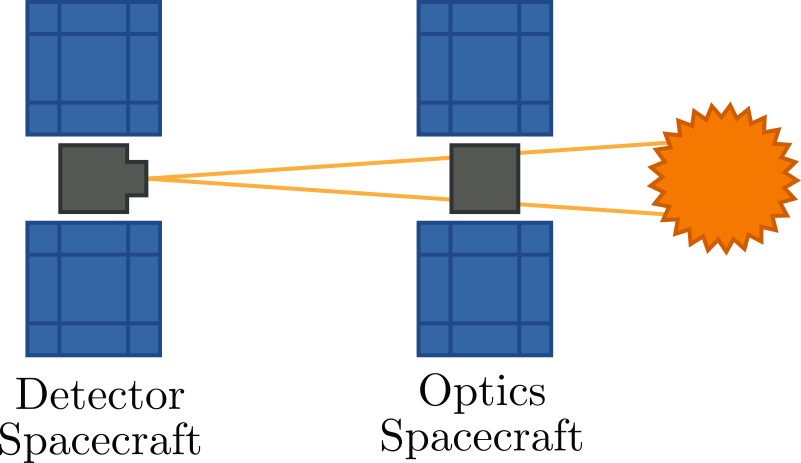
\includegraphics[width=\textwidth]{figures/visors.png}
            \caption{VISORS consists of two spacecraft, holding optics and a detector}
            \label{fig:a}
        \end{minipage}
        \hspace{0.5cm}
        \begin{minipage}[b]{0.45\linewidth}
            \centering
            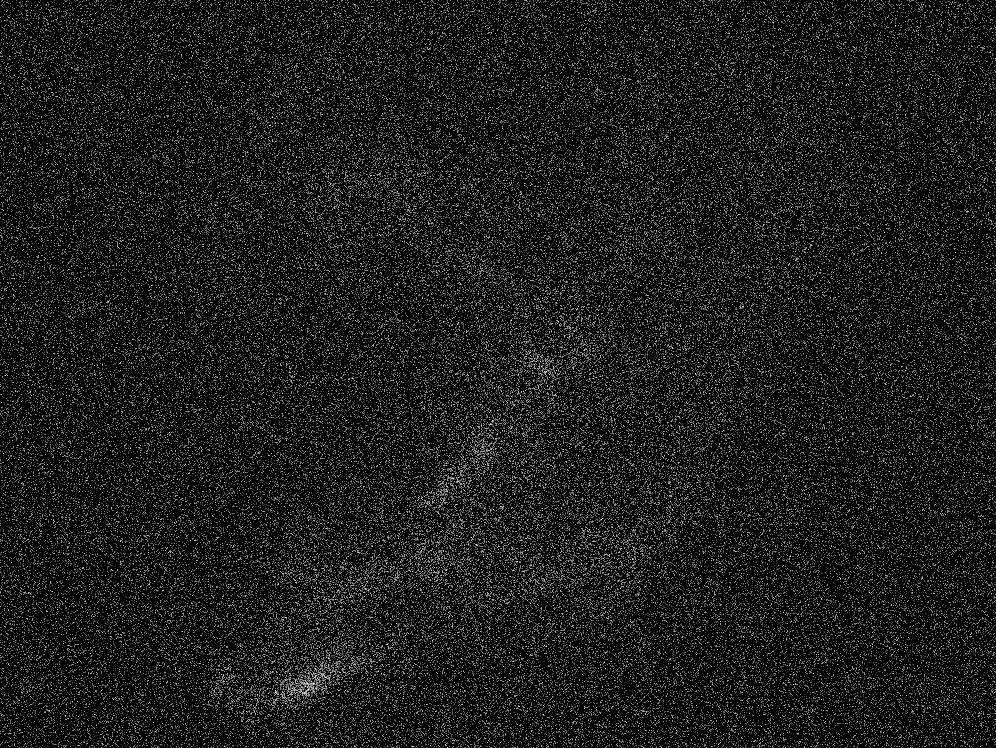
\includegraphics[width=\textwidth]{figures/sample.png}
            \caption{Example VISORS image of Sun with synthetic noise. -2.5 dB SNR}
            \label{fig:b}
        \end{minipage}
    \end{figure}

    VISORS' diffractive optics allows us to study the corona at higher resolutions, but low efficiency of the optics (7\%) can result in low SNR observations.

    We take advantage of the simple translational nature of VISORS image sequences to develop an algorithm which is maximum-likelihood optimal and performs well on low SNR observations.

  \end{block}

  \begin{block}{Observation Model}
      Let $\bm{y}_1, ..., \bm{y}_K \in \mathbb{R}^{N \times N}$ be a sequence of noisy observations where
      $$\bm{y}_k = T_{k\bm{c}}(\bm{\mu}) + \bm{n}_k$$
      \vspace*{-2cm}
      \begin{itemize}
        \item $\bm{c} \in \mathbb{R}^2$ - interframe drift
        \item $T(\cdot)$ - translation operator
        \item $\bm{u}$ - ground truth scene
        \item $\bm{n}_k \sim \mathcal{N}(0, \sigma^2)$ - additive Gaussian noise
      \end{itemize}
  \end{block}

\end{column}

\separatorcolumn

% ---------- Column 2 ----------

\begin{column}{\colwidth}


  \begin{block}{Algorithm}
    $$
    \hat{\bm{c}} = \arg\max_{\bm{c}} \sum_{m=1}^{K-1} D_m \left(
    \mathcal{F}^{-1} \left( \sum_{k=1}^{K-m} \bm{Y}_k \odot \bm{Y}_{k+m} \right)
    \right)[\bm{c}]
    $$
    \begin{center}
    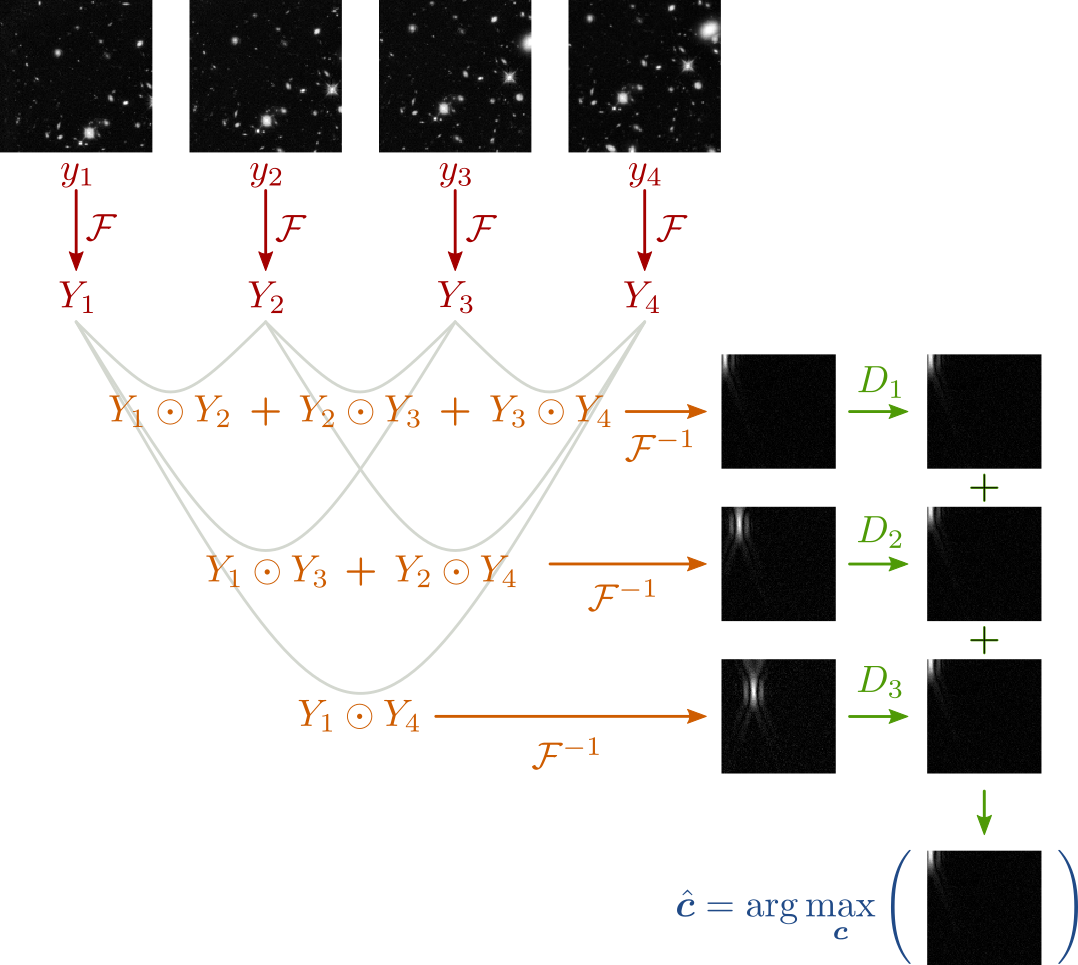
\includegraphics[width=0.9 \textwidth]{figures/algorithm.png}
    \end{center}
  \end{block}

  \begin{block}{ML Optimality - Proof Overview}
    \begin{enumerate}
    \item Derive the expression for likelihood maximization over $\bm{c}$ and $\bm{\mu}$
      $$
        \hat{\bm{c}}, \hat{\bm{\mu}} =
        \arg\min_{\bm{c}, \bm{\mu}}
        \underbrace{\sum_{k=1}^K \sum_{n=1}^N (\bm{y}_{k,n} - T_{k\bm{c}}(\bm{\mu})_n)^2}_{\text{cost}(\bm{c}, \bm{\mu})}
      $$

    \item Derive the most likely value for $\bm{\mu}$ as a function of $\bm{c}$
      $$
        \frac{d}{d\mu_j}\left(\text{cost}(\bm{c}, \bm{\mu})\right) = 0 \nonumber
        \hspace{0.5cm} \Longrightarrow \hspace{0.5cm}
        \hat{\bm{\mu}} = \sum_{k=1}^K T_{-k\bm{c}}(\bm{y}_k)
      $$
      $$\text{cost}(\bm{c}, \hat{\bm{\mu}}) = \text{cost}(\bm{c})$$

    \item Show that the log-likelihood solution consists of a sum of downsampled cross correlations

        \vspace*{-1cm}
        $$\begin{aligned}
        \hat{\bm{c}} = \arg\min_{\bm{c}} \text{cost}(\bm{c})
        &=\arg\min_{\bm{c}}\sum_{k=1}^K \sum_{n=1}^N \left(\bm{y}_{k,n} - T_{k\bm{c}}\left(\sum_{l=1}^K T_{-l\bm{c}}(\bm{y}_l)\right)_n\right)^2 \\
        &= ... = \arg\max_{\bm{c}} \sum_{m=1}^{K-1} \sum_{k=1}^{K-m} (\bm{y}_k \lstar \bm{y}_{k+m})[m\bm{c}]
        \end{aligned}$$

    \end{enumerate}
  \end{block}

\end{column}

\separatorcolumn

\begin{column}{\colwidth}

  \begin{block}{Numerical Results}
    \begin{figure}
    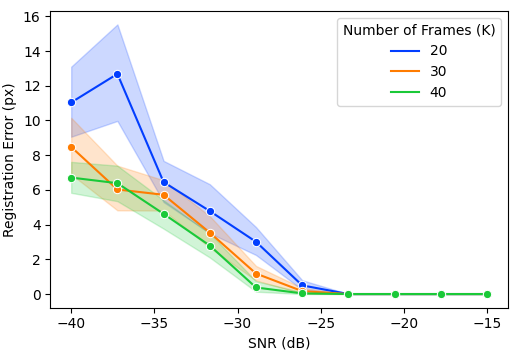
\includegraphics[width=\textwidth]{figures/db_sweep.pdf}
    \vspace*{-3cm}
    \caption{Algorithm registration error vs observation SNR}
    \end{figure}

    \begin{figure}[htb]
      \begin{minipage}[b]{.45\linewidth}
        \centering
        \centerline{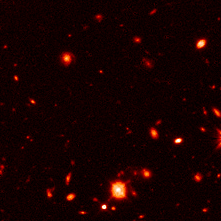
\includegraphics[width=\textwidth]{figures/recon_clean.png}}
        %  \vspace{1.5cm}
        \centerline{(a) Ground truth}\medskip
      \end{minipage}
      \hfill
      \begin{minipage}[b]{0.45\linewidth}
        \centering
        \centerline{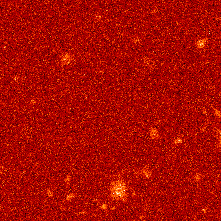
\includegraphics[width=\textwidth]{figures/recon.png}}
        %  \vspace{1.5cm}
        \centerline{(b) Fused images}\medskip
      \end{minipage}
      \caption{Ground truth and non-regularized reconstruction result for -25dB SNR AWGN and $K=30$ frames.}
      \label{fig:recon}
    \end{figure}

  \end{block}

  \vspace*{-2cm}
  \begin{block}{Future Work}
  \vspace*{-1cm}

    \begin{itemize}
      \item Algorithm implementation on STM32/FPGA
      \item Performance analysis against comparable iterative methods
    \end{itemize}

  \end{block}

  \vspace*{-1cm}
  \begin{block}{Reference}
  \vspace*{-1cm}
    \begin{itemize}
    \item E. Widloski, F. Kamalabadi ``Low SNR Multiframe Registration for Cubesats'' arXiV 2022
    \end{itemize}
  \end{block}

  Python implementation available at \href{https://github.com/evidlo/multiml}{https://github.com/evidlo/multiml}

\end{column}

\separatorcolumn
\end{columns}
\end{frame}

\end{document}
